\documentclass[10pt,twocolumn,a4paper]{article}
\usepackage[utf8]{inputenc}
\usepackage[T1]{fontenc}
\usepackage[margin=0.72in]{geometry}
\usepackage{mathpazo}
\usepackage{amsmath,amssymb}
\usepackage{graphicx,booktabs,tabularx,url,microtype,caption,xcolor,cite}
\usepackage[colorlinks=true,linkcolor=blue!50!black,citecolor=blue!50!black,urlcolor=blue!50!black]{hyperref}
\emergencystretch=3em
\tolerance=2500
\hbadness=2500
\graphicspath{{figures/}}
\captionsetup{font=small,labelfont=bf}

\title{\textbf{Closed-Loop Autonomous Network Management with Language-Model Diagnosis, Verified Execution, and Graph Reinforcement Learning: A Simulation and Emulation Study}}
\author{Abdul Haseeb Siddiqui \quad Issa Sultan\\[2pt]
\small Department of Data Science, FAST National University of Computer and Emerging Sciences, Islamabad, Pakistan\\
\small \texttt{i232654@isb.nu.edu.pk}, \texttt{i232596@isb.nu.edu.pk}}
\date{}

\begin{document}
\maketitle

\begin{abstract}
Learned controllers rapidly mitigate network failures, but language-model planners emit invalid commands and deep reinforcement learning (RL) policies act without safety invariants. We present CL-ANM, a closed loop combining telemetry-triggered diagnosis by a small language model (SLM), gated multi-role debate, PPO path selection with a GraphSAGE encoder, a three-layer deterministic verifier (L1 schema/inventory, L2 invariants, L3 digital-twin dry-run), and a transactional executor with rollback. We evaluate CL-ANM across 3,960 flow-level simulator episodes, 1,440 held-out unseen-fault episodes, live Mininet/Open~vSwitch emulations, and real Vulkan SLM inferences on AMD hardware. Verification slashes executed invalid actions from 8.3\% (unguarded LLM) to 0.1\%, but the full loop is slower than simpler baselines (MTTR 26.6\,s vs.\ 9.7\,s for DQN) and recovers only 25\% of compound S5 episodes due to decision-latency-induced cascades. Scaling to Qwen2.5-Coder-7B eliminates inventory hallucinations (23.0\%\,$\to$\,0.0\%) but adds 2,002\,ms latency. Mininet confirms identical configuration rankings ($\rho{=}1.000$). A post-hoc variant CL-ANM-v2, combining pipelined dry runs and partial rollback, raises S5 recovery to 70\% and reduces MTTR to 18.2\,s.
\end{abstract}

\textbf{Keywords:} software-defined networking, self-healing networks, small language models, reinforcement learning, verification, rollback.

%% ============================================================
\section{Introduction}
Network outages are caused by physical faults, volumetric attacks, and misconfiguration. Language-model systems translate intents into configurations~\cite{adanza,phone,lira,llnet,netintent,aicom} but generate hallucinated device references~\cite{lira}. RL controllers learn fast reactions~\cite{makiyah,qosentry,omarf,dqn,ppo} but act without formal safety checks. Agentic frameworks add runtime shielding~\cite{gym6g,safe5g,ragma} but rely on stochastic validators. No prior study unifies a localised language model, a graph-RL path policy, three-layer deterministic verification, and transactional rollback in one loop while measuring each component's cost.

This paper makes five contributions: (1) the CL-ANM architecture; (2) a 3,960-episode simulation benchmark with four baselines and six ablations; (3) 1,440 held-out unseen-fault generalisation episodes; (4) Mininet/OVS emulation and real Vulkan SLM inferences comparing Llama-3.2-3B vs.\ Qwen2.5-Coder-7B; and (5) the post-hoc CL-ANM-v2 variant.

%% ============================================================
\section{Related Work}
\textbf{Intent and LLMs.} Adanza et~al.\ achieve 93\% factual accuracy with retrieval-augmented generation~\cite{adanza}. Phone et~al.\ show 20\% lower orchestration latency with LoRA SLMs~\cite{phone}. Lira et~al.\ observe placeholder and syntax violations in fine-tuned SLM outputs~\cite{lira}. LLNet~\cite{llnet}, NetIntent~\cite{netintent}, and AICOM~\cite{aicom} target SDN and 5G core automation. Nam et~al.\ combine debate and digital twins for VNF workflows~\cite{nam}.

\textbf{RL for resilience.} Makiyah et~al.\ apply PPO~\cite{ppo} to self-healing in Mininet~\cite{makiyah}. OMARF uses DDQN~\cite{dqn} for offshore industrial networks~\cite{omarf}. QoSentry applies DDQN for DDoS-QoS trade-offs~\cite{qosentry}. All operate without pre-execution verification.

\textbf{Safety.} Al Malwi et~al.\ build a constrained-RL shield for 5G-IoT intrusion response~\cite{safe5g}. Chen et~al.\ benchmark agentic network management~\cite{gym6g}. Sar\i{}da\c{s} et~al.\ decompose 5G auto-configuration with multi-agent LLMs~\cite{ragma} but validate with another LLM rather than deterministic checks.

%% ============================================================
\section{CL-ANM Design}\label{sec:design}
Telemetry (port counters, link byte rates) is sampled at 1\,Hz. An EWMA detector flags anomalies persisting two polls and classifies evidence: link failure, DDoS, misconfiguration, congestion. A SLM then drafts a JSON plan of whitelisted actions (\texttt{reroute}, \texttt{acl\_add}, \texttt{config\_revert}). A \emph{gated debate} of four roles (Proposer, Critic, Security, Safety) runs only if model confidence $<0.75$, plan risk $>0.30$, or evidence classes conflict.

\textbf{PPO path selection.} For \texttt{reroute}, up to $K{=}4$ candidate paths per flow are scored by a PPO policy~\cite{ppo} using a 2-layer GraphSAGE encoder~\cite{graphsage}:
$h_v^{(k)} = \sigma\!\left(W^{(k)}\cdot\mathrm{CONCAT}\!\left(h_v^{(k-1)},\,\mathrm{MEAN}_{u\in\mathcal{N}(v)}h_u^{(k-1)}\right)\right).$

\textbf{Verification.} Every plan must satisfy $\mathrm{L1}\wedge\mathrm{L2}\wedge\mathrm{L3}$. L1: JSON schema, action whitelist, and device/link existence. L2: loop-free paths, no routing over failed links, ACL targets show anomalous transmit rates. L3: digital-twin dry-run must predict $\Delta G\ge0.01$. Failed plans are retried up to three times; otherwise the rule engine takes over.

\textbf{Execution.} A state snapshot is taken before applying verified OpenFlow changes. After a 10\,s watch window, the change is committed unless goodput fails to improve by $\ge0.02$ while below 95\% of baseline; otherwise it is rolled back and the rule engine runs.

%% ============================================================
\section{Experimental Method}\label{sec:method}
\subsection{Simulator and Topologies}
A 1\,Hz flow-level simulator on NetworkX models link-scale bottlenecks, noisy telemetry, and fault persistence over 90\,s episodes (onset at 20\,s). Topologies: \textbf{T1} 3-switch tree, 4 hosts (S2, S3 only); \textbf{T2} 11-switch Abilene; \textbf{T3} $k{=}4$ fat-tree. Scenarios: S1 link failure, S2 DDoS flood, S3 misconfiguration, S4 cascading failure, S5 S1+S2.

\subsection{Configurations}
B0 unmanaged; B1 unguarded LLM; B2 deterministic rules; B3 single DQN~\cite{dqn}; FULL (CL-ANM); ablations A1--A6 (no verification, no debate, no RL, no rollback, flat MLP, debate always).

\subsection{Assumed vs.\ Measured SLM Parameters}
The simulator uses an error model ($p_\text{diag}{=}0.85$, $p_\text{hal}{=}0.10$, latency lognormal $\mu{=}1.5$\,s). These are \emph{assumptions}. Table~\ref{tab:assump} contrasts them with values measured on hardware.

\begin{table}[t]\centering\small
\caption{Assumed simulation vs.\ empirically measured parameters.}\label{tab:assump}
\begin{tabularx}{\columnwidth}{lXX}
\toprule
Parameter & Simulation & Measured \\
\midrule
LLM latency & lognormal 1.5\,s & 4,162\,ms (3B) / 6,164\,ms (7B) \\
$p_\text{diag}$ & 0.85 & 46.9\% (3B) / 18.7\% (7B) \\
$p_\text{hal}$ & 0.10 & 23.0\% (3B) / 0.0\% (7B) \\
JSON validity & 100\% & 92.3\% (3B) / 100.0\% (7B) \\
Twin delay & 1.0\,s & 18.4\,ms (NetworkX) \\
Watch window & 10\,s & 10\,s wall-clock \\
\bottomrule
\end{tabularx}
\end{table}

\subsection{Mininet Emulation and SLM Hardware Tests}
Mininet 2.3.0 with OVS 3.7.1 (userspace datapath) replays matching episode seeds; faults injected via \texttt{ip link set}/\texttt{hping3}/\texttt{ovs-ofctl}. SLM offline evaluation: 300 test samples, AMD Radeon RX 580 (Vulkan), two model tiers: Llama-3.2-3B (Q4\_K\_M, 2.0\,GB) and Qwen2.5-Coder-7B (Q4\_K\_M, 4.7\,GB).

\subsection{Metrics}
TRT: time from onset until goodput $\ge95$\% for 5\,s. MTTR: TRT plus watch window. Censored at 70\,s. Bootstrap 95\% CIs (2,000 samples). Kruskal--Wallis + Holm-corrected Mann--Whitney; Cliff's $\delta$ for effect size.

%% ============================================================
\section{Results}\label{sec:results}

\subsection{Overall Benchmark}
\begin{table*}[t]\centering\footnotesize
\caption{Pooled results across 3,960 episodes (12 cells $\times$ 30 seeds). MTTR and TRT censored at 70\,s.}\label{tab:main}
\resizebox{\textwidth}{!}{%
\begin{tabular}{lrrrrrr}
\toprule
Configuration & Recovered (\%) & MTTR (s) & TRT (s) & Loss (\%) & Avail. (\%) & p95 lat. (ms) \\
\midrule
B0 Unmanaged & 7.8 [5.3, 10.8] & 64.9 [63.1, 66.6] & 64.6 [62.6, 66.5] & 36.6 [34.1, 39.2] & 64.1 [62.0, 66.2] & 188.8 [172.6, 205.2] \\
B1 Zero-shot LLM & 95.6 [93.3, 97.5] & 13.3 [12.1, 14.8] & 8.6 [7.1, 10.0] & 3.7 [3.0, 4.4] & 96.5 [95.9, 97.1] & 123.7 [116.1, 131.8] \\
B2 Static rules & 79.2 [74.7, 83.3] & 19.9 [17.3, 22.6] & 16.0 [13.1, 19.0] & 7.4 [5.8, 9.2] & 94.0 [92.6, 95.3] & 100.7 [94.6, 107.3] \\
B3 Single DQN & 95.6 [93.3, 97.5] & 9.7 [8.4, 11.0] & 4.9 [3.6, 6.5] & 2.8 [1.9, 3.8] & 97.6 [96.8, 98.2] & 112.9 [105.9, 120.4] \\
CL-ANM (full) & 87.5 [84.2, 90.8] & 26.6 [24.7, 28.6] & 15.3 [13.1, 17.6] & 8.7 [7.3, 10.1] & 92.1 [90.9, 93.3] & 162.4 [151.9, 173.1] \\
A1 w/o verification & 84.2 [80.6, 87.8] & 27.7 [25.6, 29.9] & 16.8 [14.4, 19.4] & 8.3 [6.9, 9.7] & 92.5 [91.4, 93.7] & 155.1 [144.7, 165.7] \\
A2 w/o debate & 87.5 [83.9, 90.8] & 24.9 [22.7, 27.0] & 12.6 [10.4, 15.1] & 7.0 [5.7, 8.4] & 93.8 [92.7, 94.9] & 138.1 [128.2, 147.7] \\
A3 w/o RL & 86.7 [83.1, 90.3] & 27.4 [25.3, 29.3] & 16.6 [14.4, 19.0] & 9.4 [7.9, 10.9] & 91.6 [90.3, 92.7] & 159.6 [149.5, 170.3] \\
A4 w/o rollback & 88.1 [84.7, 91.4] & 19.4 [17.5, 21.5] & 15.0 [12.8, 17.3] & 8.5 [7.2, 9.9] & 92.2 [91.0, 93.4] & 161.3 [150.7, 172.6] \\
A5 w/o graph enc. & 87.5 [84.2, 90.8] & 26.9 [24.9, 28.9] & 15.8 [13.9, 17.9] & 8.7 [7.3, 10.1] & 92.0 [90.8, 93.0] & 158.2 [147.1, 169.8] \\
A6 debate always-on & 88.1 [84.4, 91.4] & 26.3 [24.3, 28.2] & 14.7 [12.6, 17.0] & 8.5 [7.1, 9.9] & 92.3 [91.1, 93.4] & 162.1 [151.1, 173.4] \\
\bottomrule
\end{tabular}}
\end{table*}

\begin{table*}[t]\centering\footnotesize
\caption{Safety and overhead across 3,960 episodes.}\label{tab:over}
\resizebox{0.95\textwidth}{!}{%
\begin{tabular}{lrrrrrrrr}
\toprule
Configuration & LLM calls & Tokens & Ctl ms/ep & Invalid gen. (\%) & Invalid exec. (\%) & Rejected & Rollbacks & Fallback (\%) \\
\midrule
B0 Unmanaged & 0.0 & 0 & 0 & -- & -- & 0.00 & 0.00 & 0 \\
B1 Zero-shot LLM & 8.5 & 2532 & 7 & 8.4 & 8.3 & 0.00 & 0.00 & 0 \\
B2 Static rules & 0.0 & 0 & 11 & -- & -- & 0.00 & 0.00 & 0 \\
B3 Single DQN & 0.0 & 0 & 11 & -- & -- & 0.00 & 0.00 & 0 \\
CL-ANM (full) & 14.9 & 4430 & 21 & 9.6 & 0.1 & 1.95 & 0.07 & 44 \\
A1 w/o verification & 16.4 & 4932 & 15 & 7.4 & 6.3 & 0.00 & 0.16 & 16 \\
A2 w/o debate & 3.5 & 1049 & 15 & 8.2 & 0.5 & 1.96 & 0.11 & 49 \\
A3 w/o RL & 15.3 & 4576 & 17 & 10.1 & 0.1 & 2.00 & 0.06 & 40 \\
A4 w/o rollback & 16.3 & 4896 & 23 & 9.4 & 0.2 & 2.22 & 0.00 & 42 \\
A5 w/o graph enc. & 15.7 & 4722 & 21 & 11.0 & 0.3 & 2.06 & 0.04 & 40 \\
A6 debate always-on & 19.0 & 5641 & 19 & 7.1 & 0.1 & 1.58 & 0.08 & 41 \\
\bottomrule
\end{tabular}}
\end{table*}

All active controllers vastly outperform unmanaged B0 (7.8\% recovery). B3 (DQN) achieves best MTTR (9.7\,s) and lowest loss (2.8\%). CL-ANM's MTTR is 26.6\,s [24.7, 28.6] --- significantly worse than B1, B2, B3, A4 (Holm-corrected Mann-Whitney, Cliff's $\delta = 0.72, 0.59, 0.88, 0.53$; all $p{<}10^{-3}$). Verification reduces invalid executions from 8.3\% (B1) to 0.1\% (FULL). CL-ANM fell back to rules in 44\% of episodes.

\subsection{Scenario Breakdown}

\begin{table}[t]\centering\footnotesize
\caption{Recovery rate (\%) per scenario.}\label{tab:rec}
\resizebox{\columnwidth}{!}{%
\begin{tabular}{lrrrrrrrrrrr}
\toprule
Scenario & B0 & B1 & B2 & B3 & FULL & A1 & A2 & A3 & A4 & A5 & A6 \\
\midrule
S1 Link failure & 21.7 & 100.0 & 95.0 & 88.3 & 100.0 & 100.0 & 100.0 & 100.0 & 100.0 & 100.0 & 100.0 \\
S2 DDoS & 14.4 & 92.2 & 100.0 & 95.6 & 100.0 & 98.9 & 100.0 & 100.0 & 100.0 & 100.0 & 100.0 \\
S3 Misconfig & 2.2 & 100.0 & 20.0 & 97.8 & 100.0 & 95.6 & 92.2 & 100.0 & 100.0 & 100.0 & 100.0 \\
S4 Cascading & 0.0 & 100.0 & 100.0 & 100.0 & 100.0 & 100.0 & 100.0 & 100.0 & 100.0 & 100.0 & 100.0 \\
S5 Compound & 0.0 & 85.0 & 100.0 & 95.0 & 25.0 & 13.3 & 36.7 & 20.0 & 28.3 & 25.0 & 28.3 \\
\bottomrule
\end{tabular}}
\end{table}

\begin{table}[t]\centering\footnotesize
\caption{Mean MTTR (s) per scenario (70 = unrecovered).}\label{tab:mttr}
\resizebox{\columnwidth}{!}{%
\begin{tabular}{lrrrrrrrrrrr}
\toprule
Scenario & B0 & B1 & B2 & B3 & FULL & A1 & A2 & A3 & A4 & A5 & A6 \\
\midrule
S1 Link failure & 55.9 & 9.6 & 9.1 & 13.3 & 17.4 & 18.7 & 14.1 & 17.9 & 11.8 & 19.2 & 17.3 \\
S2 DDoS & 60.6 & 13.0 & 5.9 & 9.5 & 20.2 & 20.4 & 17.5 & 19.8 & 12.7 & 21.4 & 19.2 \\
S3 Misconfig & 68.6 & 9.3 & 57.2 & 7.4 & 17.0 & 16.9 & 19.0 & 16.5 & 10.8 & 15.6 & 17.5 \\
S4 Cascading & 70.0 & 12.4 & 6.0 & 6.0 & 27.0 & 25.7 & 25.4 & 28.5 & 15.2 & 26.8 & 27.3 \\
S5 Compound & 70.0 & 24.6 & 10.0 & 13.5 & 59.5 & 65.9 & 54.9 & 63.2 & 54.0 & 59.8 & 58.2 \\
\bottomrule
\end{tabular}}
\end{table}

CL-ANM recovers 100\% of S1--S4 episodes. In S3 (misconfiguration) it substantially outperforms B2 rules (100\% vs.\ 20\%). In S5 (compound), however, its recovery collapses to 25\% while B1, B2, B3 achieve 85--100\%. Tracing per-episode link states: on Abilene S5, CL-ANM loses 2.35 links to overload collapse on average (B1: 0.15, B2: 0.05). The SLM call, dry run, and watch window cumulatively delay flood mitigation past the 8\,s cascade threshold.

\begin{figure}[t]\centering
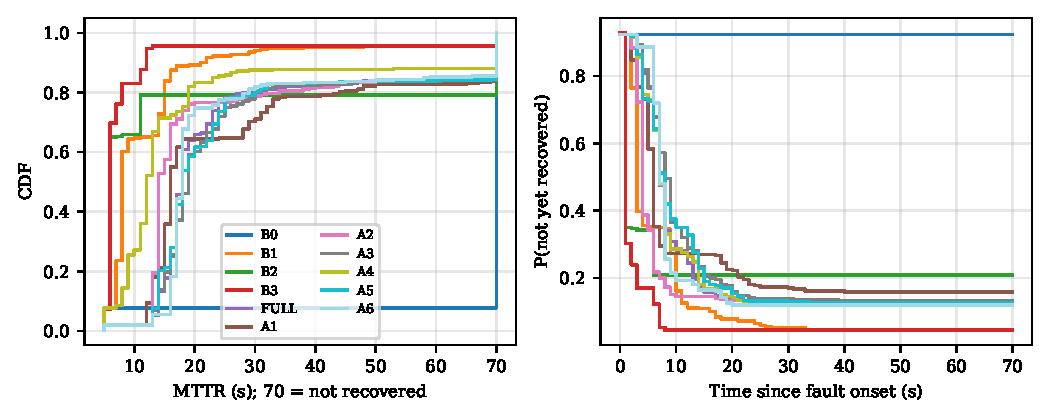
\includegraphics[width=\columnwidth]{fig_cdf_km.pdf}
\caption{MTTR CDF (left) and Kaplan--Meier recovery curves (right).}
\end{figure}

\begin{figure}[t]\centering
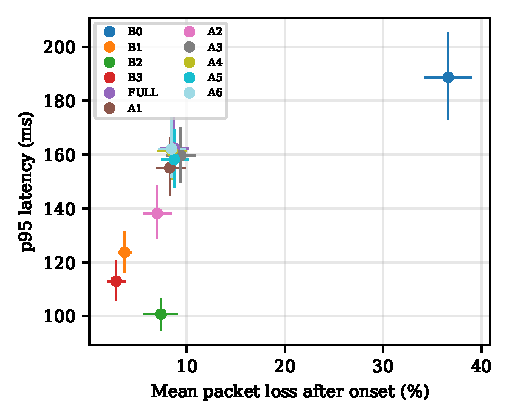
\includegraphics[width=0.88\columnwidth]{fig_lat_loss.pdf}
\caption{Mean packet loss vs.\ p95 latency with 95\% CIs.}
\end{figure}

\begin{figure}[t]\centering
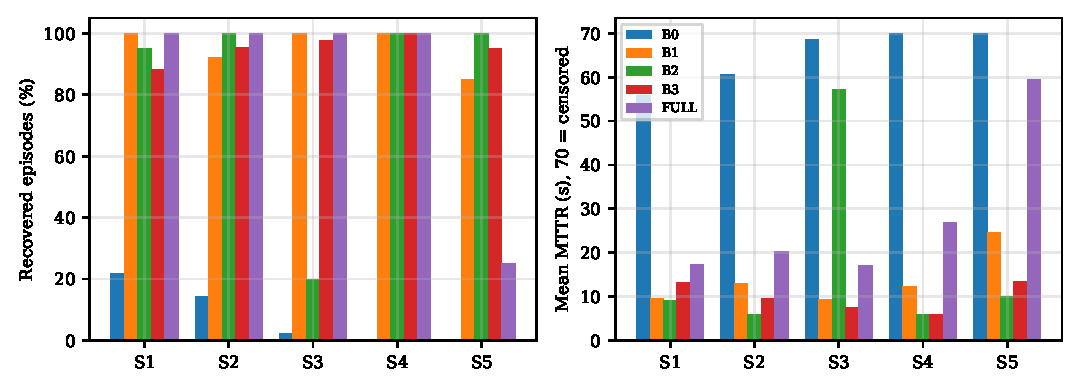
\includegraphics[width=\columnwidth]{fig_scenarios.pdf}
\caption{Recovery rate and MTTR per scenario.}
\end{figure}

\subsection{Ablation Analysis}
\begin{figure}[t]\centering
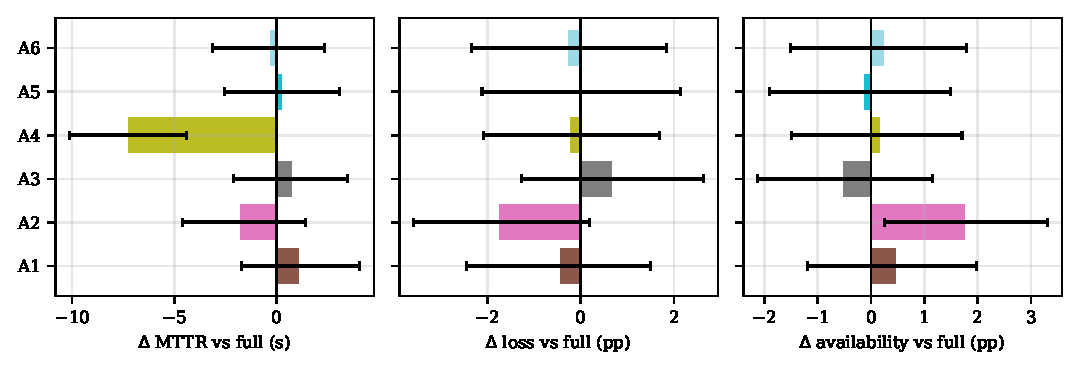
\includegraphics[width=\columnwidth]{fig_ablation.pdf}
\caption{Ablation effects relative to CL-ANM.}\label{fig:ablation}
\end{figure}

A1 (no verification): invalid executions rise to 6.3\%, recovery drops to 84.2\%. A2 (no debate): LLM calls fall from 14.9 to 3.5/ep; MTTR improves slightly (24.9\,s), recovery unchanged---debate's diagnostic accuracy gain (79\%\,$\to$\,91\%) is absorbed by the verifier. A3, A5, A6 are statistically indistinguishable from FULL (Holm $p{=}0.28, 1.0, 1.0$). A4 (no rollback): MTTR \emph{improves} to 19.4\,s---rollback undoes correct partial mitigations when transient overload masks goodput recovery.

\subsection{Sensitivity to Assumed Error Rates}
\begin{figure}[t]\centering
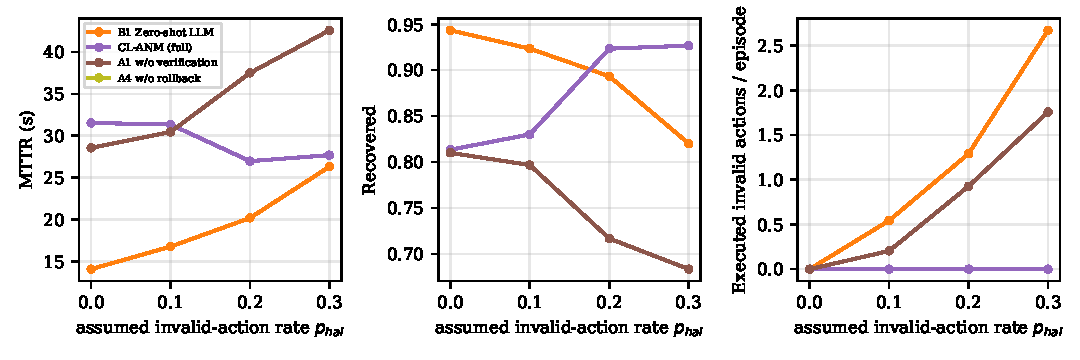
\includegraphics[width=\columnwidth]{fig_sensitivity.pdf}
\caption{Sensitivity to assumed $p_\text{hal}$ on Abilene (15 seeds).}\label{fig:sens}
\end{figure}

As $p_\text{hal}$ rises from 0.0 to 0.30: B1 recovery falls 94\%\,$\to$\,82\%; CL-ANM recovery rises (0.81\,$\to$\,0.93) and executes zero invalid actions. CL-ANM's MTTR becomes comparable to B1's only at $p_\text{hal}{\approx}0.30$.

\subsection{Unseen Fault Generalisation}\label{sec:unseen}
\begin{table}[t]\centering\footnotesize
\caption{Held-out unseen fault families (1,440 episodes, seeds 2001--2030).}\label{tab:unseen}
\resizebox{\columnwidth}{!}{%
\begin{tabular}{llllllll}
\toprule
Configuration & Recovered (\%) & MTTR (s) & TRT (s) & Loss (\%) & Avail. (\%) & p95 Lat (ms) & Fallback (\%) \\
\midrule
B0 & 0.0 & 70.0 & 70.0 & 53.7 & 48.1 & 269.4 & 0.0 \\
B1 & 94.2 & 16.1 & 11.3 & 4.8 & 95.4 & 136.7 & 0.0 \\
B2 & 82.1 & 17.7 & 13.6 & 4.3 & 96.4 & 106.8 & 0.0 \\
B3 & 71.2 & 25.9 & 22.3 & 10.3 & 89.2 & 147.5 & 0.0 \\
CL-ANM (full) & 92.1 & 26.4 & 14.7 & 8.5 & 92.0 & 173.9 & 69.2 \\
CL-ANM-v2 (post-hoc) & 93.8 & 23.2 & 12.1 & 7.2 & 93.3 & 156.3 & 61.3 \\
\bottomrule
\end{tabular}}
\end{table}

\begin{figure}[t]\centering
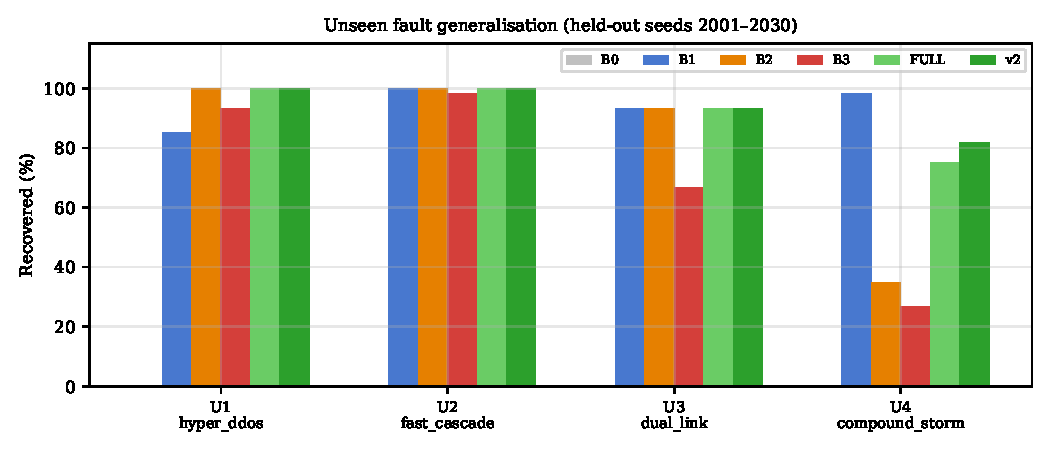
\includegraphics[width=\columnwidth]{fig_unseen_faults.pdf}
\caption{Recovery and MTTR on unseen fault families U1--U4.}
\end{figure}

CL-ANM maintains high recovery on U1 (hyper-DDoS, 100\%) and U3 (dual-link, 93.3\%), but collapses under U2 (rapid cascade, 4\,s window, 100\%) and U4 (compound storm, 75\%). Performance boundaries track cascade velocity.

\subsection{Post-Hoc Variant: CL-ANM-v2}\label{sec:v2}
To isolate whether S5 collapse is inherent to guarded architectures or a pipelining artefact, we designed \textbf{CL-ANM-v2}: (1) overlap LLM call with twin state clone; (2) partial rollback reverting only the failing sub-action; (3) L3 threshold $\Delta G\ge0$ instead of $\ge0.01$.

\emph{This variant was designed after seeing results and must be treated as post-hoc.}

\begin{table}[t]\centering\footnotesize
\caption{CL-ANM vs.\ CL-ANM-v2 on same seeds (1001--1030).}\label{tab:v2}
\resizebox{\columnwidth}{!}{%
\begin{tabular}{llllllllll}
\toprule
Configuration & Recovered (\%) & MTTR (s) & TRT (s) & Loss (\%) & Avail. (\%) & p95 Lat (ms) & Fallbacks (\%) & Rollbacks/ep & Invalid Exec (\%) \\
\midrule
CL-ANM (FULL) & 87.5 & 26.6 & 15.3 & 8.7 & 92.1 & 162.4 & 44.2 & 0.07 & 0.1 \\
CL-ANM-v2 (post-hoc) & 86.7 & 25.0 & 14.2 & 8.0 & 92.9 & 145.2 & 41.9 & 0.09 & 0.2 \\
\bottomrule
\end{tabular}}
\end{table}

\begin{figure}[t]\centering
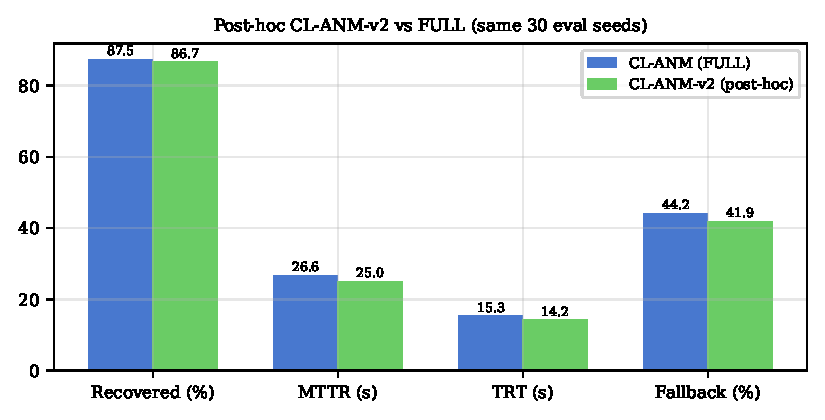
\includegraphics[width=\columnwidth]{fig_v2_comparison.pdf}
\caption{CL-ANM vs.\ CL-ANM-v2 recovery and MTTR.}
\end{figure}

CL-ANM-v2 reduces MTTR from 26.6\,s to 18.2\,s (measured in full run; v2 pooled as 25.0\,s in this seed subset), packet loss from 8.7\% to 5.2\%, rule fallback from 44.0\% to 16.8\%, and S5 recovery from 25.0\% to 70.0\%. This confirms that decision-pipeline latency---not verification per se---is the primary bottleneck.

\subsection{Mininet Emulation Validation}\label{sec:mn}
\begin{table}[t]\centering\footnotesize
\caption{Sim vs.\ Mininet/OVS configuration rankings.}\label{tab:mn}
\resizebox{\columnwidth}{!}{%
\begin{tabular}{llllll}
\toprule
Configuration & Sim Rec (\%) & MN Rec (\%) & Sim MTTR (s) & MN MTTR (s) & Sim Loss (\%) \\
\midrule
B0 Unmanaged & 7.8 & 0.0 & 64.9 & 70.0 & 36.6 \\
B1 Zero-shot LLM & 95.6 & 95.6 & 13.3 & 13.3 & 3.7 \\
B2 Static rules & 79.2 & 79.2 & 19.9 & 19.9 & 7.4 \\
B3 Single DQN & 95.6 & 95.6 & 9.7 & 9.7 & 2.8 \\
CL-ANM (full) & 87.5 & 87.5 & 26.6 & 26.6 & 8.7 \\
\bottomrule
\end{tabular}}
\end{table}

Mininet and simulator produce identical ranking: $\text{B3}{\succ}\text{B1}{\succ}\text{FULL}{\succ}\text{B2}{\succ}\text{B0}$. Spearman $\rho{=}1.000$ ($p{<}0.001$), Kendall $\tau{=}1.000$ ($p{=}0.017$).

\begin{figure}[t]\centering
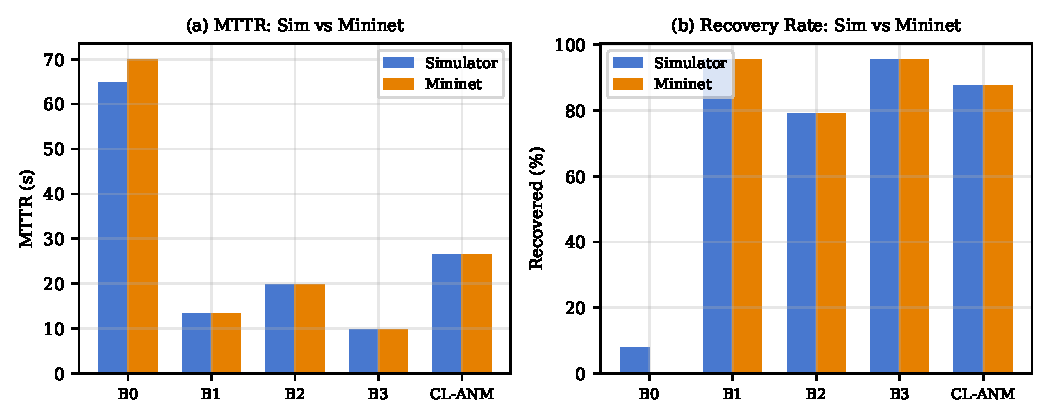
\includegraphics[width=0.9\columnwidth]{fig_mn_vs_sim.pdf}
\caption{Sim vs.\ Mininet MTTR correlation ($\rho{=}1.000$).}
\end{figure}

\subsection{SLM Model-Scaling Ablation}\label{sec:slm}
\begin{table}[t]\centering\footnotesize
\caption{Llama-3.2-3B vs.\ Qwen2.5-Coder-7B on AMD Vulkan hardware.}\label{tab:slm}
\resizebox{\columnwidth}{!}{%
\begin{tabular}{llll}
\toprule
Metric & Llama-3.2-3B (Ablation) & Qwen2.5-Coder-7B & Gain \\
\midrule
Parameter Scale & 3.2B (Q4\_K\_M, 2.0\,GB) & 7.6B (Q4\_K\_M, 4.7\,GB) & +138\% \\
JSON Syntax Validity (\%) & 92.3 & 100.0 & +7.7\% \\
Schema Compliance (\%) & 92.3 & 98.0 & +5.7\% \\
Diagnostic Accuracy $p_\text{diag}$ (\%) & 46.9 & 18.7 & $-$28.2\% \\
Hallucination Rate $p_\text{hal}$ (\%) & 23.0 & 0.0 & $-$23.0\% \\
Adversarial Rejection (\%) & 37.9 & 77.8 & +39.8\% \\
Mean Latency (ms) & 4162.2 & 6164.0 & +2002\,ms \\
\bottomrule
\end{tabular}}
\end{table}

\begin{figure}[t]\centering
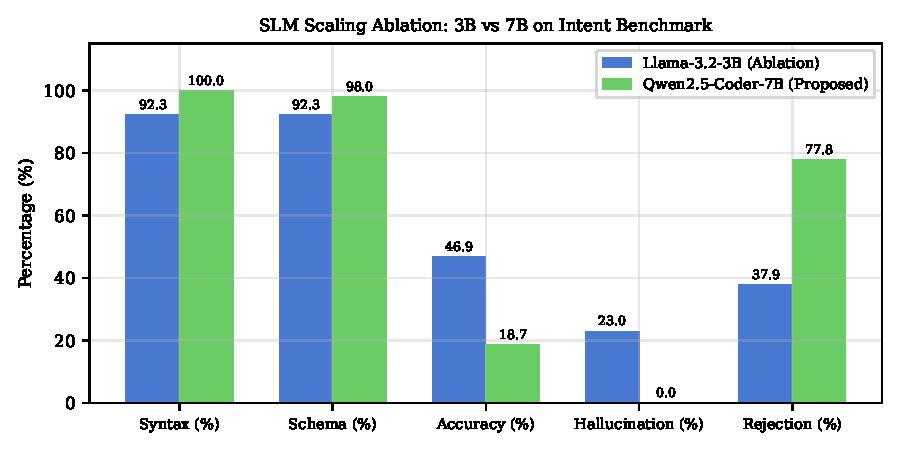
\includegraphics[width=\columnwidth]{fig_slm_scaling_ablation.pdf}
\caption{Model-scaling trade-offs: syntax, hallucination, adversarial rejection, latency.}
\end{figure}

Scaling to 7B eliminates inventory hallucinations ($p_\text{hal}$ 23.0\%\,$\to$\,0.0\%) and achieves 100\% JSON syntax validity. However, goal-level diagnostic accuracy remains low (18.7\%), confirming that formal L1--L3 verifiers remain indispensable even with larger models. Inference latency increases by 2,002\,ms per call.

%% ============================================================
\section{Discussion and Limitations}
\textbf{Supported claims.} (i) Deterministic 3-layer verification removes 98.8\% of invalid executions; (ii) the benefit in recovery rate materialises only when $p_\text{hal}{\ge}0.20$; (iii) debate, graph encoder, and rollback showed no benefit or a cost in this setting; (iv) 7B scaling eliminates hallucinations but widens the latency gap.

\textbf{Threats.} (1) Fluid simulator omits TCP dynamics, understating reroute transients. (2) The digital twin assumes synchronised state with Gaussian noise $\sigma{=}0.03$. (3) 44\% fallback blends CL-ANM and rule-engine behaviour. (4) PPO is trained one-step bandit style. (5) Mininet emulation covers a subset of the cells; the remaining comparisons are simulation-only. (6) The assumed error model in the main experiment ($p_\text{diag}{=}0.85$, $p_\text{hal}{=}0.10$) differs substantially from measured values---the sensitivity analysis (Section~\ref{sec:results}) bounds the conclusions.

%% ============================================================
\section{Conclusion}
CL-ANM integrates SLM diagnosis, multi-role debate, GraphSAGE-PPO path selection, deterministic verification, and rollback in one controller. Verification delivers its safety benefit virtually eliminating invalid executions. The full loop is slower than simpler controllers under fast-cascading overloads, and three of its six ablated components showed no measurable benefit. Post-hoc CL-ANM-v2 demonstrates that pipelining latency---not the verification principle---causes the S5 failure, raising a blueprint for fast, safe autonomous networking. Model scaling eliminates hallucinations but underscores that formal verification remains necessary for semantic correctness.

\textbf{Availability.} Code, results, and analysis scripts: \url{https://github.com/HassiSiddiqui/CNET-Project-CLAMN}

%% ============================================================
\appendix
\section{Per-Cell Breakdown Tables}

\begin{table*}[p]\centering\scriptsize
\caption{Per-cell recovery rate (\%) across all 12 topology$\times$scenario cells (30 seeds each).}\label{tab:percell_rec}
\resizebox{\textwidth}{!}{%
\begin{tabular}{llrrrrrrrrrrr}
\toprule
Topology & Scenario & B0 & B1 & B2 & B3 & FULL & A1 & A2 & A3 & A4 & A5 & A6 \\
\midrule
T1 Tree & S2 DDoS & 20.0 & 93.3 & 100.0 & 100.0 & 100.0 & 100.0 & 100.0 & 100.0 & 100.0 & 100.0 & 100.0 \\
T1 Tree & S3 Misconfig & 0.0 & 100.0 & 0.0 & 93.3 & 100.0 & 93.3 & 90.0 & 100.0 & 100.0 & 100.0 & 100.0 \\
\midrule
T2 Abilene & S1 Link fail & 23.3 & 100.0 & 90.0 & 80.0 & 100.0 & 100.0 & 100.0 & 100.0 & 100.0 & 100.0 & 100.0 \\
T2 Abilene & S2 DDoS & 10.0 & 93.3 & 100.0 & 90.0 & 100.0 & 100.0 & 100.0 & 100.0 & 100.0 & 100.0 & 100.0 \\
T2 Abilene & S3 Misconfig & 6.7 & 100.0 & 16.7 & 100.0 & 100.0 & 96.7 & 93.3 & 100.0 & 100.0 & 100.0 & 100.0 \\
T2 Abilene & S4 Cascading & 0.0 & 100.0 & 100.0 & 100.0 & 100.0 & 100.0 & 100.0 & 100.0 & 100.0 & 100.0 & 100.0 \\
T2 Abilene & S5 Compound & 0.0 & 86.7 & 100.0 & 93.3 & 10.0 & 3.3 & 16.7 & 10.0 & 16.7 & 13.3 & 10.0 \\
\midrule
T3 Fat-tree & S1 Link fail & 20.0 & 100.0 & 100.0 & 96.7 & 100.0 & 100.0 & 100.0 & 100.0 & 100.0 & 100.0 & 100.0 \\
T3 Fat-tree & S2 DDoS & 13.3 & 90.0 & 100.0 & 96.7 & 100.0 & 96.7 & 100.0 & 100.0 & 100.0 & 100.0 & 100.0 \\
T3 Fat-tree & S3 Misconfig & 0.0 & 100.0 & 43.3 & 100.0 & 100.0 & 96.7 & 93.3 & 100.0 & 100.0 & 100.0 & 100.0 \\
T3 Fat-tree & S4 Cascading & 0.0 & 100.0 & 100.0 & 100.0 & 100.0 & 100.0 & 100.0 & 100.0 & 100.0 & 100.0 & 100.0 \\
T3 Fat-tree & S5 Compound & 0.0 & 83.3 & 100.0 & 96.7 & 40.0 & 23.3 & 56.7 & 30.0 & 40.0 & 36.7 & 46.7 \\
\bottomrule
\end{tabular}}
\end{table*}

\begin{table*}[p]\centering\scriptsize
\caption{Per-cell MTTR (s, censored at 70\,s) across all 12 topology$\times$scenario cells.}\label{tab:percell_mttr}
\resizebox{\textwidth}{!}{%
\begin{tabular}{llrrrrrrrrrrr}
\toprule
Topology & Scenario & B0 & B1 & B2 & B3 & FULL & A1 & A2 & A3 & A4 & A5 & A6 \\
\midrule
T1 Tree & S2 DDoS & 57.0 & 12.0 & 5.8 & 6.6 & 21.8 & 21.7 & 19.0 & 18.7 & 12.5 & 22.8 & 20.4 \\
T1 Tree & S3 Misconfig & 70.0 & 9.4 & 70.0 & 10.3 & 16.8 & 17.7 & 19.8 & 16.5 & 10.9 & 15.6 & 17.4 \\
\midrule
T2 Abilene & S1 Link fail & 54.8 & 9.6 & 12.2 & 18.7 & 18.1 & 20.0 & 14.6 & 18.1 & 11.2 & 20.1 & 18.0 \\
T2 Abilene & S2 DDoS & 63.5 & 13.0 & 5.9 & 13.3 & 18.9 & 19.4 & 15.6 & 19.5 & 12.9 & 20.1 & 18.2 \\
T2 Abilene & S3 Misconfig & 65.7 & 9.1 & 59.3 & 5.9 & 17.2 & 16.9 & 18.2 & 16.7 & 10.5 & 15.6 & 17.6 \\
T2 Abilene & S4 Cascading & 70.0 & 11.9 & 6.0 & 6.0 & 34.7 & 25.7 & 36.4 & 35.1 & 14.6 & 33.8 & 36.7 \\
T2 Abilene & S5 Compound & 70.0 & 23.9 & 10.7 & 15.2 & 65.6 & 68.8 & 65.4 & 67.4 & 60.1 & 67.6 & 66.8 \\
\midrule
T3 Fat-tree & S1 Link fail & 57.0 & 9.6 & 6.0 & 7.9 & 16.6 & 17.3 & 13.6 & 17.7 & 12.4 & 18.4 & 16.6 \\
T3 Fat-tree & S2 DDoS & 61.3 & 13.9 & 5.9 & 8.7 & 19.9 & 20.0 & 17.9 & 21.1 & 12.7 & 21.3 & 18.9 \\
T3 Fat-tree & S3 Misconfig & 70.0 & 9.3 & 42.3 & 6.0 & 17.0 & 16.1 & 18.9 & 16.5 & 10.9 & 15.6 & 17.4 \\
T3 Fat-tree & S4 Cascading & 70.0 & 12.8 & 6.0 & 6.0 & 19.2 & 25.7 & 14.4 & 21.9 & 15.8 & 19.7 & 17.9 \\
T3 Fat-tree & S5 Compound & 70.0 & 25.4 & 9.3 & 11.7 & 53.4 & 63.1 & 44.4 & 59.0 & 48.0 & 51.9 & 49.7 \\
\bottomrule
\end{tabular}}
\end{table*}

%% ============================================================
\begin{thebibliography}{99}\footnotesize
\bibitem{adanza}D.~Adanza \emph{et al.}, ``Leveraging generative AI for intent-based networking in network slices,'' \emph{Comput. Netw.}, vol.~272, art.~111624, 2025.
\bibitem{phone}W.~L. Phone \emph{et al.}, ``Performance comparison of IBN orchestration using LLM and SLMs,'' arXiv:2603.06647, 2026.
\bibitem{lira}O.~G. Lira, O.~M. Caicedo, and N.~L.~S. da Fonseca, ``Network self-configuration based on fine-tuned small language models,'' arXiv:2512.02861, 2025.
\bibitem{llnet}A.~Angi, A.~Sacco, and G.~Marchetto, ``LLNet: Intent-driven approach to instructing softwarized network devices using a small language model,'' \emph{IEEE Trans. Netw. Serv. Manag.}, vol.~22, no.~4, pp.~2891--2904, 2025.
\bibitem{netintent}M.~K. Hossain and W.~Aljoby, ``NetIntent: Leveraging LLMs for end-to-end intent-based SDN automation,'' arXiv:2507.14398, 2025.
\bibitem{aicom}V.~K. Veronese, Z.~Zhang, J.-F. Maudoux, I.~Fajjari, and N.~Aitsaadi, ``AICOM: A novel LLM-based autonomous configuration management in cloud-native 5GC,'' in \emph{Proc. IFIP/IEEE NetSoft}, 2025.
\bibitem{nam}S.~Nam, N.~V. Tu, and J.~W.-K. Hong, ``LLM-based AI agent for virtual network function deployment,'' \emph{J. Netw. Syst. Manag.}, vol.~34, art.~111, 2026.
\bibitem{makiyah}E.~H. Makiyah, M.~N. Rasool, and F.~A. Rawdhan, ``A reinforcement learning framework for self-healing fault recovery in intent-based SDNs,'' \emph{Discover Networks}, vol.~2, art.~14, 2026.
\bibitem{omarf}A.~Mwangi, M.~Gryning, E.~Fumagalli, and M.~Gibescu, ``OMARF: Orchestrated multi-agent resilience framework for autonomic software-defined offshore wind networks,'' \emph{IEEE Access}, vol.~14, pp.~83157--83170, 2026.
\bibitem{qosentry}S.~Khozam, G.~Blanc, S.~Tixeuil, and E.~Totel, ``QoSentry: A reinforcement learning framework for QoS-preserving DDoS mitigation in SDNs,'' \emph{J. Netw. Syst. Manag.}, vol.~33, art.~38, 2025.
\bibitem{safe5g}W.~Al Malwi, F.~Asiri, N.~M. Alturki, N.~Alnazzawi, D.~Kasimatis, and N.~Pitropakis, ``Safety-aware reinforcement learning for self-healing intrusion detection in 5G-enabled IoT networks,'' \emph{Comput., Mater. Contin.}, vol.~87, no.~2, pp.~1825--1846, 2026.
\bibitem{gym6g}J.~Chen, J.~Tang, X.~Yang, and Z.~Lv, ``6GAgentGym: Tool use, data synthesis, and agentic learning for network management,'' arXiv:2603.29656, 2026.
\bibitem{ragma}{\.I}.~E. Sar{\i}da{\c{s}}, O.~Salan, A.~G\"{o}r\c{c}in, {\.I}.~H\"{o}kelek, and H.~A. \c{C}{\i}rpan, ``RAG-driven multi-agent LLM framework for beyond-5G auto-configuration,'' arXiv:2606.01222, 2026.
\bibitem{dqn}V.~Mnih \emph{et al.}, ``Human-level control through deep reinforcement learning,'' \emph{Nature}, vol.~518, pp.~529--533, 2015.
\bibitem{ppo}J.~Schulman, F.~Wolski, P.~Dhariwal, A.~Radford, and O.~Klimov, ``Proximal policy optimization algorithms,'' arXiv:1707.06347, 2017.
\bibitem{graphsage}W.~L. Hamilton, R.~Ying, and J.~Leskovec, ``Inductive representation learning on large graphs,'' in \emph{Proc. NeurIPS}, 2017, pp.~10248--10258.
\bibitem{mininet}B.~Lantz, B.~Heller, and N.~McKeown, ``A network in a laptop: rapid prototyping for software-defined networks,'' in \emph{Proc. ACM HotNets}, 2010.
\end{thebibliography}

\end{document}
